\documentclass[10pt,letterpaper]{article}

\usepackage{cogsci}
\usepackage{pslatex}
\usepackage{apacite}
\usepackage{graphicx}
\usepackage{algorithmic}

%% wrap algorithm in a figure environment without caption and number.
%% #1 is the title of the algorithm.
\newenvironment{myalgorithm}[1]%
{\begin{figure}[!h]\small\noindent\rule{\linewidth}{1pt}\\#1\vspace{-0.5em}\\%
\rule{\linewidth}{0.5pt}\\\vspace{-1em}}%
{\vspace{-0.5em}\rule{\linewidth}{1pt}\end{figure}}

\title{Contour Representation and Shape Matching \\Based on Mechanism of Visual Cortex}
 
\author{{\large \bf Hui Wei (weihui@fudan.edu.cn)} \\
  School of Computer Science, Fudan University \\
  Shanghai, 200437 China
  \AND {\large \bf Zheng Dong (dongzheng@fudan.edu.cn)} \\
  School of Computer Science, Fudan University \\
  Shanghai, 200437 China}


\begin{document}

\maketitle


\begin{abstract}
We present a novel model to represent and match contour lines of closed shapes.
This model is based on the mechanism of visual cortex.
It extracts orientation features from input images with simple computation units 
that imitate simple cells in the visual cortex.
The contour lines are accurately located by searching adjacent activated simple units.
These activated simple units are concatenated in a chain to code the contour lines of closed shapes.
In order to match between shapes, we propose a measure based on Fr\'echet distance
and use dynamic programming to calculate the distance between different chains of simple units.
The model is evaluated on the MPEG7 shape data set.
We also demonstrate that this model can explain the shape selectivity of visual area V4.


\textbf{Keywords:} 
contour representation; shape matching; simple cells; visual cortex
\end{abstract}


\section{Introduction}

Shape matching is a central problem in visual information system, computer vision, 
pattern recognition and robotics. 
Traditional studies of shape matching make use of image transformation and computation geometry 
\cite{veltkamp2001}.
The robustness and efficiency of these methods are far from perfection compared with human vision.
Recent studies on the neural system of vision have accumulated sufficient knowledge 
and inspiration for us to understand shape recognition in the biological vision
\cite{gustavsen2003,pasupathy2002}.
In this paper, we investigate into the biological vision system
and propose a novel model for curve representation and shape matching.

The proposed model extracts orientation features from input images 
with simple computation units which imitate simple cells in the visual cortex.
The contour lines of closed shapes are then accurately located by
searching through adjacent activated simple units.
These adjacent activated simple units are concatenated in a chain 
to code the contour lines.
To measure the difference between contour lines, we propose a modified version of Fr\'echet distance
\cite{alt2003}.
The distance between chains of simple units are then calculated efficiently 
with a dynamic programming approach.

The proposed model is evaluated with shape retrieval experiment on the MPEG7 shape data set.
The experiment result shows that, by the nature of this model, 
its representation of contour lines is invariant in both location and scale.
Although the performance of shape retrieval on certain data set can still be improved,
we demonstrate that, more importantly,
this model can explain the shape selectivity found in some of the neurons in cortical area V4, 
which plays a significant role in the visual pathway for object recognition in the brain.

\section{Neural Mechanism of Vision}

\subsection{Ganglion Cells and Simple Cells}

Visual stimuli projected to the retina are transformed into neural impulses
by the retina ganglion cells \cite{enroth1966}.
Ganglion cells are known for the concentric arrangement of their receptive fields,
which can be modeled as Difference of Gaussian (DoG) filters
(\figurename~\ref{fig:1}).
They are sensitive to contrast in their receptive fields.

Neural impulses from ganglion cells are passed on through lateral geniculate nucleus (LGN)
to simple cells in the primary visual cortex (V1) \cite{hubel1962}.
Simple cells respond to oriented edges (light bar, dark bar, or boundary between the two).
The receptive field of simple cell is usually modeled as a Gabor function.
It is composed of elongated excitatory area and inhibitory area.
This kind of receptive field is formed by summation of the receptive fields of ganglion cells
\cite{reid1995}.
Every simple cell receives output of several ganglion cells, of which the receptive fields
are lined up in an elongated band (\figurename~\ref{fig:1}).

\begin{figure}[ht]
\begin{center}
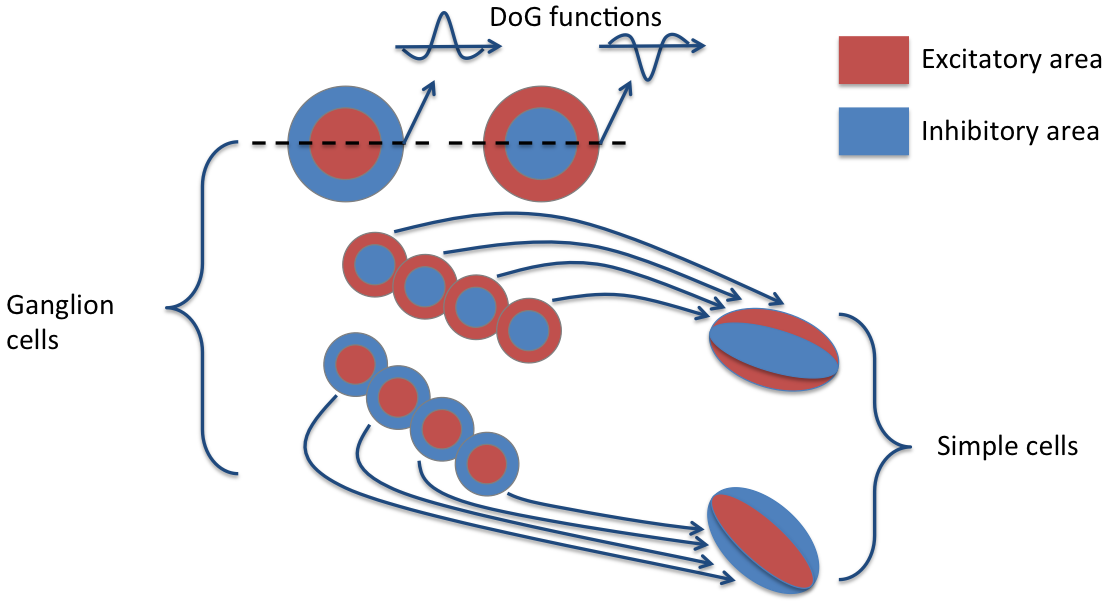
\includegraphics[width=0.95\linewidth]{images/fig1.png}
\end{center}
\caption{Receptive fields of ganglion cells and simple cells.} 
\label{fig:1}
\end{figure}

Visual information processing in the brain follows a hierarchical scheme.
Higher level in the visual cortex extracts information by aggregating its low-level input.
Simple cells aggregate output of ganglion cells arranged in line.
In our proposed model, we aggregate output of simple cells to form our representation of contour lines.

\subsection{Ventral Visual Pathway}

Primate brains possess two distinct visual systems. 
As visual information exits the occipital lobe, it follows two main pathways \cite{ettlinger1990}.
The dorsal pathway terminates in the parietal lobe 
and it is involved with processing the object's spatial location relevant to the viewer. 
The ventral pathway (\figurename~\ref{fig:2})
travels to the temporal lobe and is involved with object discrimination and recognition. 
Lower levels of the pathway (visual area V1 and V2) extract features such as edges and orientations. 
At the final stages in IT cortex, neurons tend to selectively respond to complex objects 
like faces and body parts \cite{bell2009}.
Shape recognition is in the intermediate level of the pathway, visual area V4 \cite{pasupathy2002}.

\begin{figure}[ht]
\begin{center}
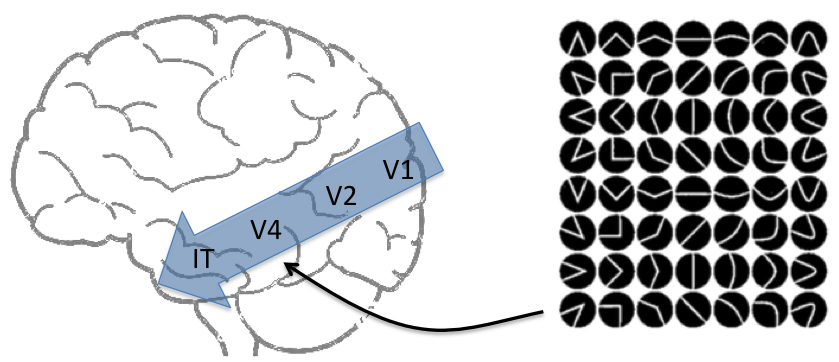
\includegraphics[width=0.95\linewidth]{images/fig2.png}
\end{center}
\caption{The ventral visual pathway and V4 patterns.} 
\label{fig:2}
\end{figure}

It is suggested that V4 processes information about contour features 
as a step toward complex shape recognition \cite{pasupathy1999}.
The right side of \figurename~\ref{fig:2} shows some of the patterns 
used in biological experiment to examine the selectivity of V4 neurons.
We will demonstrate that our model has the capacity to distinguish these patterns.

\section{Representation of Contour Lines}

We propose a novel model inspired by visual cortex.
It extracts orientation features from input images
and accurately locate contour lines, which are further encoded
with chains of simple units.
The contour lines represented in chains of simple units 
can be compared with Fr\'echet distance efficiently
in a dynamic programming approach.
Shape matching is achieved by finding the minimal Fr\'echet distance
between the representation of contour lines.

\subsection{Orientation Columns}

Cortical column is the basic functional unit in the cortex.
In the primary visual cortex, an orientation column contains
simple cells with different preferred orientations \cite{hubel1962}.
These simple cells have adjacent or overlapped receptive fields.
Therefore, an orientation column can accurately detect edges
and determine orientation of edges within a limited region of the visual field.

\begin{figure}[ht]
\begin{center}
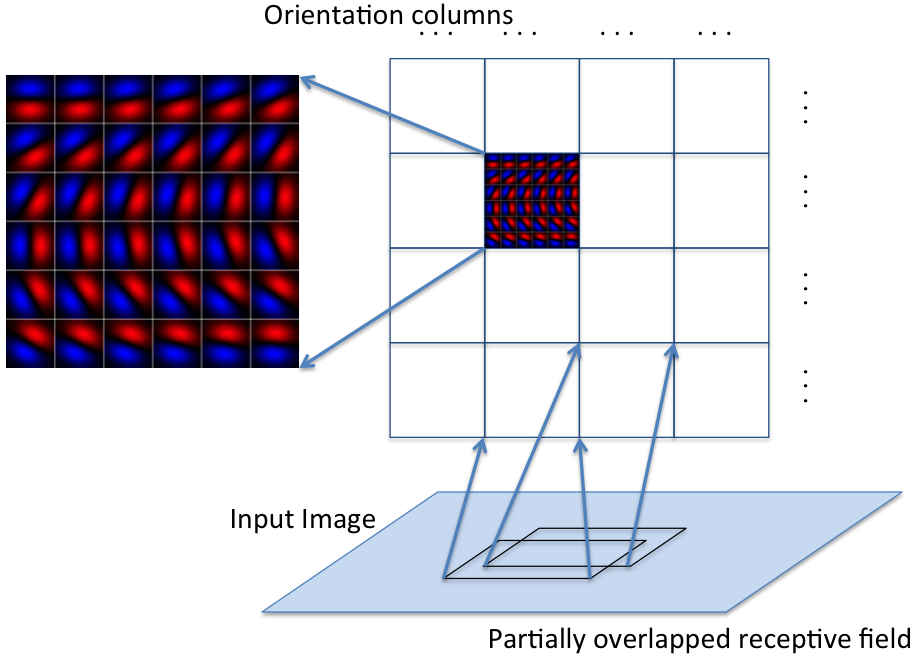
\includegraphics[width=0.95\linewidth]{images/fig3.png}
\end{center}
\caption{Orientation columns.} 
\label{fig:3}
\end{figure}

In our model, orientation columns are organized in rectangular grid
(\figurename~\ref{fig:3}).
Each column contains 36 simple computation units corresponding to 
simple cells with different preferred orientations.
Their preferred orientations cover from $0^\circ$ to $175^\circ$ in steps of $5^\circ$.
All simple units within the same column share the same receptive field in the input image.
In our experiment, the size of the receptive field is $9\times 9$ in pixels.
Neighboring columns have partially overlapped receptive fields
which move by $1$ pixel horizontally and/or vertically.

The simple computation units are modeled with the Gabor filter \cite{gabor1946}.
It is defined as follows.

\begin{equation}\label{equ:1}
g_{\theta}(x,y)
=\exp \left(-\frac{x'^2+y'^2}{2\sigma_s^2}\right)
\sin \left(2\pi\frac{x'}{\lambda}\right),
\end{equation}
where $x'=x\cos\theta+y\sin\theta$, $y'=-x\sin\theta+y\cos\theta$.
In the equation, $\theta$ represents the preferred orientation,
$\sigma_s$ approximates the radius of the receptive fields,
and $\lambda$ is the wavelength of the sinusoidal factor.
$\lambda$ controls the spatial frequency of the filter.
In this paper, it is taken according to the scale of the filter
($\lambda=1.3\sigma_s$).

The output of simple units is a convolution of the Gabor filter and the input image.

\begin{equation}\label{equ:2}
S_{\theta}=\left|\sum_{(x,y)\in RF}I(x,y)\cdot g_{\theta}(x,y)\right|,
\end{equation}
where $S_{\theta}$ is the output of the simple unit with preferred orientation $\theta$,
$I$ is the image, and $RF$ is the receptive field.

Within a single orientation column, a ``winner-takes-all'' strategy is adopted.
Only the simple unit with the maximum output value gets the chance to be activated.
A threshold is also used to ignore those units with comparatively low values.

\subsection{Locating Contour Lines}

The response map of the orientation columns shows the contour lines of the input image.
To accurately locate these contour lines, we have to find ridges in the response map
(\figurename~\ref{fig:4}(a)).
The ridges of a smooth function of two variables are a set of curves 
whose points are local maxima of the function in at least one dimension.
We use a computation network (demonstrated in \figurename~\ref{fig:4}(b)) to calculate ridge points.

\begin{figure}[ht]
\begin{center}
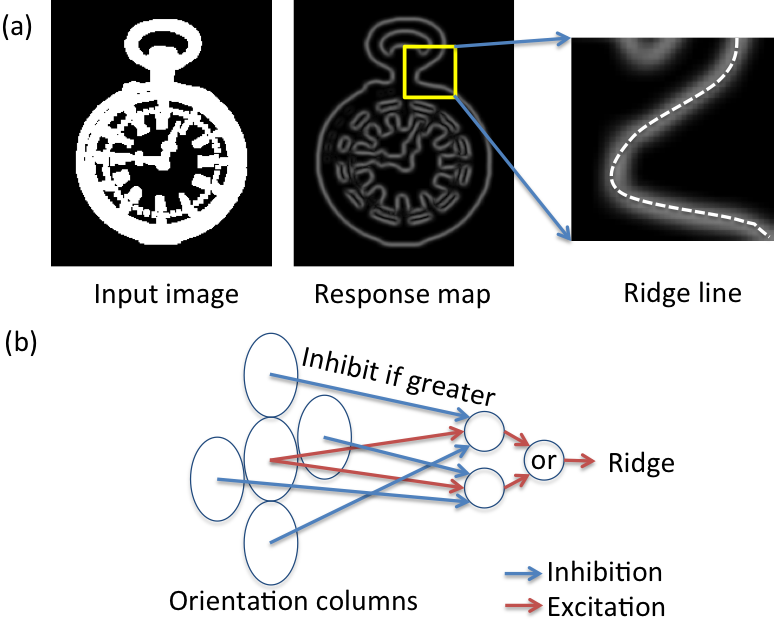
\includegraphics[width=0.95\linewidth]{images/fig4.png}
\end{center}
\caption{(a) Contour line is at ridges of response map.
(b) Computation network for ridge detection.} 
\label{fig:4}
\end{figure}

Given an input image, we get a response map of activated simple units in the orientation columns.
Ridge points are then detected. Each ridge point corresponds to an activated simple unit
and thus it has a preferred orientation which also indicates the orientation of the ridge.
Let $V$ be the set of activated simple units at the ridge points.
Function $f:V\rightarrow[0,\pi)$ is the orientation of the simple units.
If we can find an ordered set $P\subset V$ which contains all the simple units along the contour line,
then $(P,f)$ forms a representation of the contour of the shape in the input image.

\begin{figure}[ht]
\begin{center}
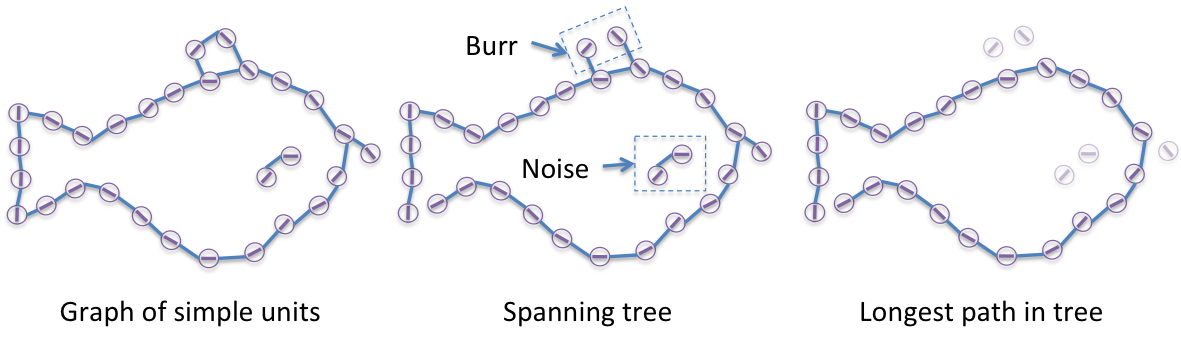
\includegraphics[width=0.99\linewidth]{images/fig5.png}
\end{center}
\caption{Finding longest path in the graph of simple units.} 
\label{fig:5}
\end{figure}

Let $\epsilon$ be the threshold of minimal distance between adjacent simple units.
Taking $V$ as a vertex set, we can construct graph $G=(V,E)$, where the edge set is
\begin{equation}\label{equ:3}
E=\{(v_1,v_2)|v_1\in V,v_2\in V,d(v_1,v_2)\le\epsilon\}
\end{equation}
The function $d(\cdot,\cdot)$ is the distance between two simple units.
Finding the longest path in a graph is known to be NP-hard (reducing from Hamiltonian path problem).
To simplify the computation, we get an arbitrary spanning tree of the graph
and find the longest path in the tree in polynomial time with the following algorithm
(proof of correctness in \cite{bulterman2002}).

\begin{myalgorithm}{Algorithm 1 LongestPathInTree}
\begin{algorithmic}[1]
\STATE Let $V_T$ be the vertex set of the tree
\STATE Pick an arbitrary vertex $v_1$ from $V_T$
\STATE Let $v_1$ be the root node of the tree
\STATE Find deepest leaf node $v_2$ by traversing from root
\STATE Let $v_2$ be the root node of the tree
\STATE Find deepest leaf node $v_3$ by traversing from root
\RETURN Path from $v_2$ to $v_3$
\end{algorithmic}
\end{myalgorithm}

As shown in \figurename~\ref{fig:5},
by finding the longest path of the spanning tree,
the main contour lines are reserved.
The noise and burr along the contour are ignored by this algorithm.

\begin{figure}[ht]
\begin{center}
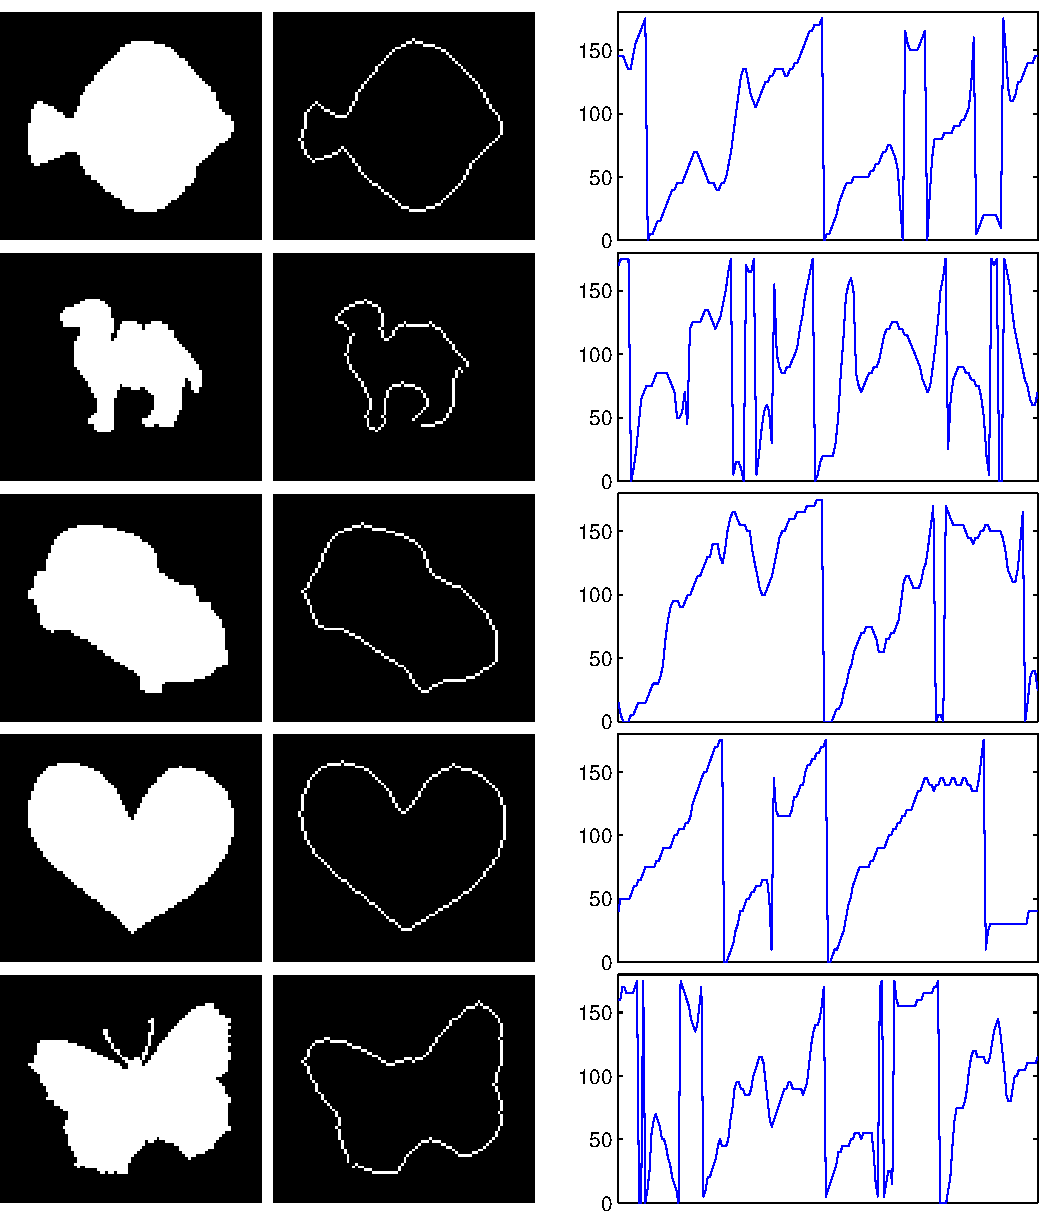
\includegraphics[width=0.99\linewidth]{images/fig6.pdf}
\end{center}
\caption{Contour representation. 
From left to right: the first column shows the original image;
the second column shows the longest path;
the third column shows the orientation of simple units along the path.} 
\label{fig:6}
\end{figure}

We demonstrate some examples of shapes represented in our model (\figurename~\ref{fig:6}).
These shapes are taken from the MPEG-7 shape data set \cite{jeannin1999}.
The shapes are represented with our model as chains of activated simple units
along the longest path of contour lines.

\section{Matching Closed Shapes}

In this section, we provide a method for matching closed shapes represented with our model.
The contour line of a closed shape is usually a cyclic path.
To make comparison between shapes, we first align their contour lines in acyclic paths.
Then we define the Fr\'echet distance \cite{alt1995} between different paths
and use the free space diagram \cite{alt2003}
to provide an efficient dynamic programming algorithm to compute the distance.

\subsection{Contour Alignment and Fr\'echet Distance}

We use the following algorithm to align the contour line.
The algorithm first find the most top-left point $s$
and the most top-right point $t$.
It then return the realigned path that starts from $s$ and goes first through $t$
(\figurename~\ref{fig:7}).

\begin{myalgorithm}{Algorithm 2 AlignContourLine}
\begin{algorithmic}[1]
\STATE Let $P=\{(x_1,y_1),(x_2,y_2),\cdots,(x_n,y_n)\}$ be coordinates of the simple units along the contour
\STATE Find $s$ such that $x_s^2+y_s^2\le x_i^2+y_i^2$ for $i=1,2,\cdots,n$
\STATE Find $t$ such that $y_t-x_t\le y_i-x_i$ for $i=1,2,\cdots,n$
\IF{$(t-s)\mathop\mathrm{mod}n\ge n/2$}
  \STATE Let $s\leftarrow n - s + 1$
  \STATE Reverse the path $P$
\ENDIF
\STATE Let $P_1\leftarrow\{(x_s,y_s),(x_{s+1},y_{s+1}),\cdots,(x_n,y_n)\}$
\STATE Let $P_2\leftarrow\{(x_1,y_1),(x_2,y_2),\cdots,(x_{s-1},y_{s-1})\}$
\RETURN $P_1 + P_2$
\end{algorithmic}
\end{myalgorithm}

\begin{figure}[ht]
\begin{center}
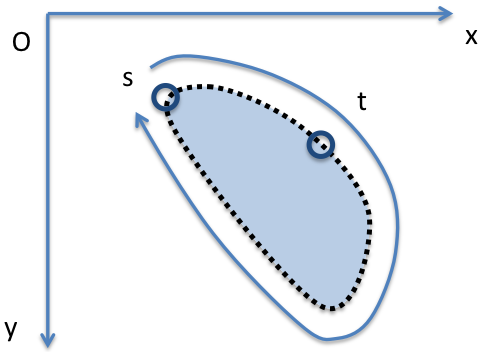
\includegraphics[width=0.5\linewidth]{images/fig7.png}
\end{center}
\caption{Contour alignment.} 
\label{fig:7}
\end{figure}

We now give a formal definition of the discrete Fr\'echet distance between 
contour lines represented in the form of simple unit chains.
Let $P=\{p_1,p_2,\cdots,p_m\}$ and $Q=\{q_1,q_2,\cdots,q_n\}$ represent two chains of simple units.
Let $f(p_i)$ and $f(q_j)$ represent the preferred orientation of the simple units.

We define a coupling of two integer sequence $\{1,2,\cdots,m\}$ and $\{1,2,\cdots,n\}$
as a pair of non-decreasing integer functions $\alpha:[1,t]\rightarrow[1,m]$ and $\beta:[1,t]\rightarrow[1,n]$
such that:

(1) $t\ge m$ and $t\ge n$;

(2) $\alpha(1) = \beta(1) = 1$, $\alpha(t) = m$ and $\beta(t) = n$;

(3) $\alpha(i+1)\le\alpha(i)+1$ and $\beta(i+1)\le\beta(i)+1$ for any $i=1,2,\cdots,t-1$.

Then the discrete Fr\'echet distance between $P$ and $Q$ is defined as follows.
\begin{equation}\label{equ:4}
F(P,Q)=\inf_{\alpha,\beta}\sum_{i=1}^{t}|f(p_{\alpha(i)})-f(q_{\beta(i)})|.
\end{equation}

When we compute the absolute difference of orientations,
we always take the smaller of the two intersection angles.
In our definition, we do not take maximal value over difference
as that is usually defined in a general definition of Fr\'echet distance.
Instead, we take summation to suppress the impact of noise.

\subsection{Free Space Diagram and Dynamic Programming}

Free space diagram (\figurename~\ref{fig:8}) is a two dimensional diagram.
The value at coordinate $(u,v)$ is the distance between the point $u$ in one path
and the point $v$ in the other path.
In our case, the value is the difference of preferred orientations of the corresponding simple units.
With free space diagram, computing Fr\'echet distance is converted into a problem of
finding a path from the top-left corner to the bottom-right corner of the two dimensional diagram.
In the case of our model, the path is the one with the minimal sum of values
and it shall only go towards the bottom or the right.
In the demonstration shown in \figurename~\ref{fig:8}, the path is colored in light green.

\begin{figure}[ht]
\begin{center}
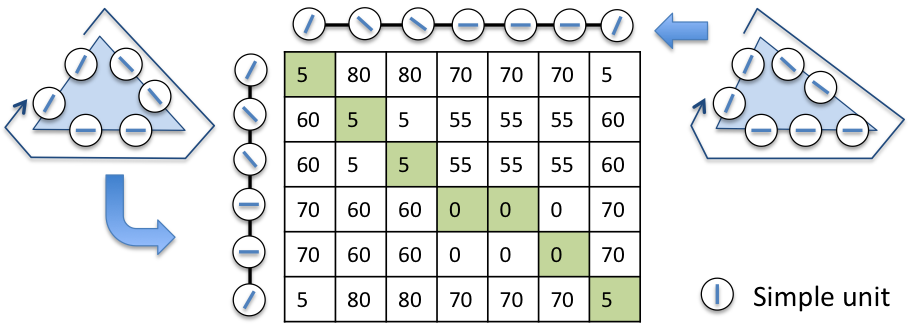
\includegraphics[width=0.95\linewidth]{images/fig8.png}
\end{center}
\caption{Free space diagram of two simple unit chains.} 
\label{fig:8}
\end{figure}

We provide a dynamic programming algorithm to compute Fr\'echet distance from the free space diagram.
Let $P_i$ be a sub-chain of the first $i$ simple units in $P$.
Let $Q_j$ be a sub-chain of the first $j$ simple units in $Q$.
We use $F_{i,j}$ to denote the Fr\'echet distance of $P_i$ and $Q_j$.
Let $M_{i,j}$ represent the value at the $i$-th row and $j$-th column in the free space diagram. 
The dynamic programming algorithm is based on the following recurrence relation.
\begin{equation}\label{equ:5}
F_{i,j}=
\left\{\begin{array}{ll}
M_{1,1} & \mbox{ if $i=j=1$}\\
M_{i,j} + F_{i,j-1} & \mbox{ if $i=1$}\\
M_{i,j} + F_{i-1,j} & \mbox{ if $j=1$}\\
M_{i,j} + \min\{F_{i-1,j},F_{i,j-1},F_{i-1,j-1}\} & \mbox{ otherwise}
\end{array}\right.
\end{equation}

With the recurrence relation in equation (\ref{equ:5}),
we can calculate the Fr\'echet distance and in the free space diagram we simultaneously construct a path
of which the summation is the Fr\'echet distance (like the light green path in \figurename~\ref{fig:8}).
This path shows a match between the simple units of the two chains
and hence a match between the contour lines.

\subsection{Shape Matching}

We use images from the MPEG-7 shape data set to demonstrate shape matching with our model.
\figurename~\ref{fig:9} shows some examples of the match between different shapes.
By the nature of our model,
the simple unit chain representation of contour lines is invariant to changes in position and scale.
The demonstration shows clearly this kind of invariance.

\begin{figure}[ht]
\begin{center}
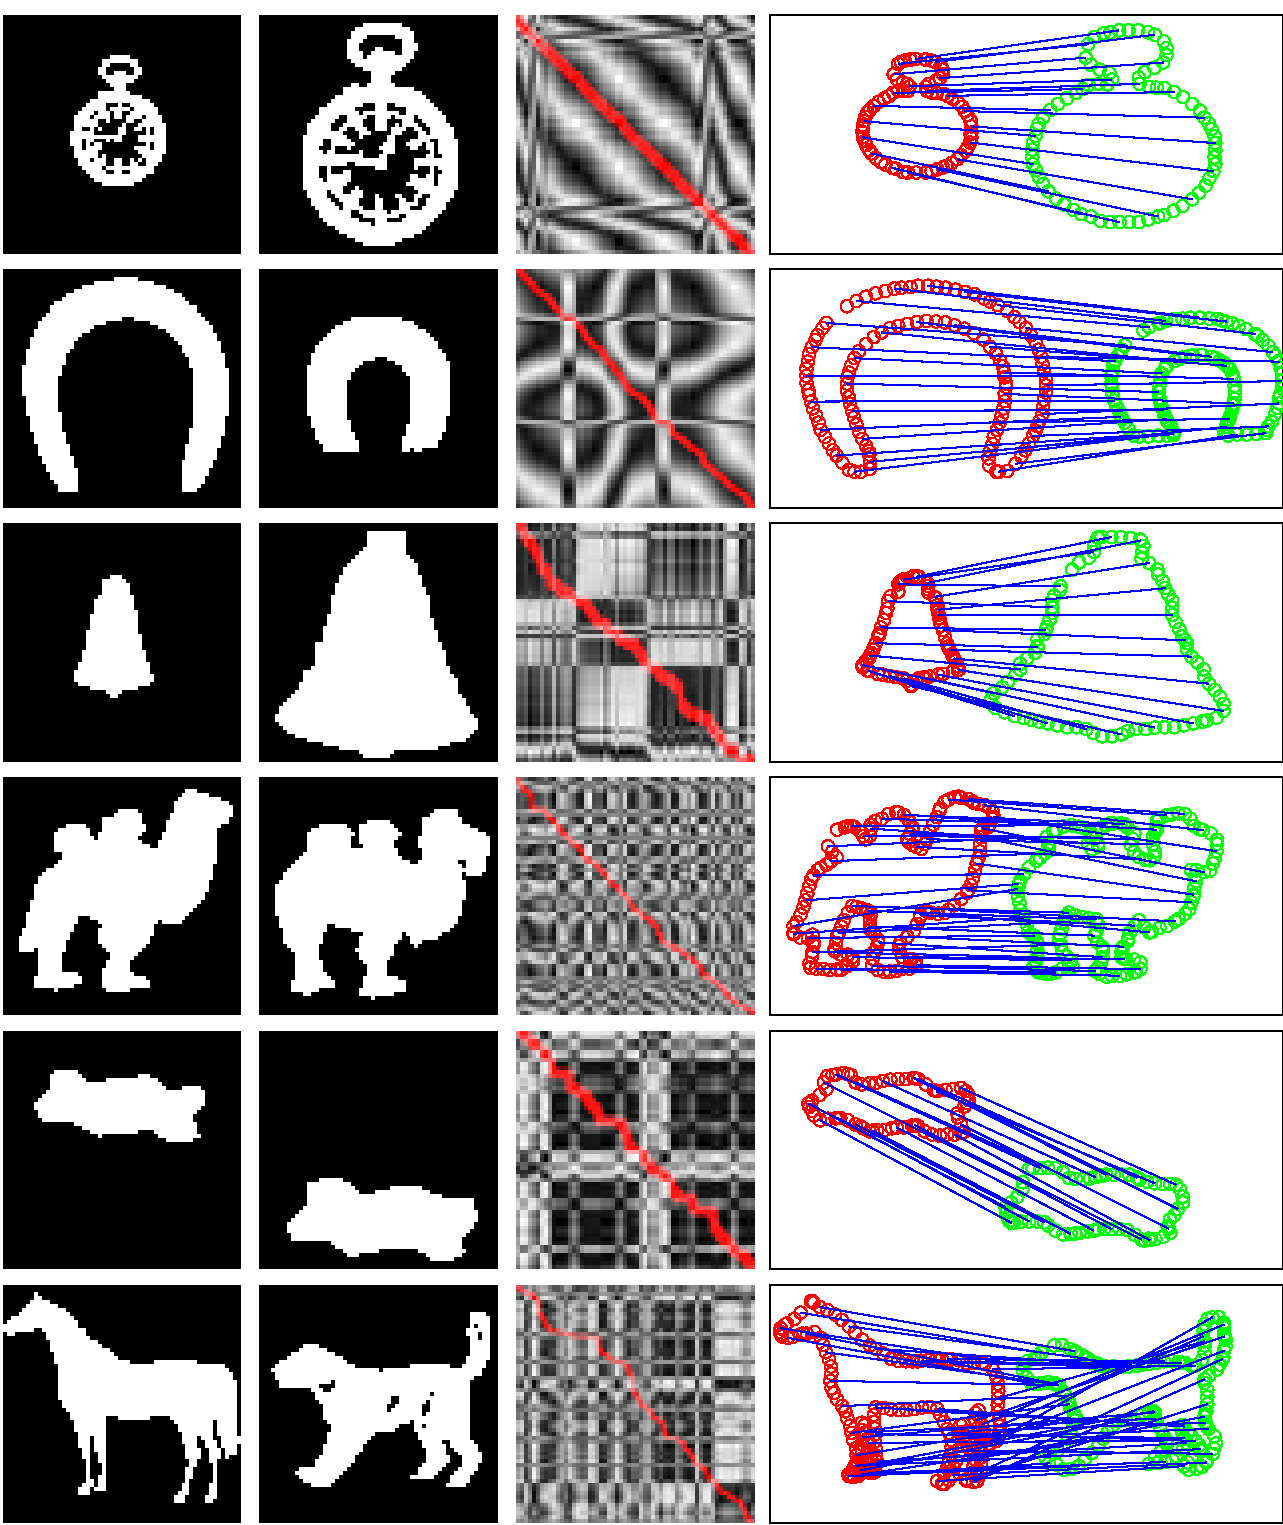
\includegraphics[width=1\linewidth]{images/fig9.pdf}
\end{center}
\caption{Shape matching result.
From left to right: the first two columns are the original images;
the third column is the free space diagram;
the fourth column shows match between shapes.} 
\label{fig:9}
\end{figure}

In \figurename~\ref{fig:9},
we paint the free space diagram in the third column.
Gray scale indicates the value in the free space diagram.
Red lines show the paths which sum to the Fr\'echet distance and indicate match between the shapes.
The first three rows demonstrate match between similar shapes in different scale.
The fourth row shows match between two shapes of camels with small discrepancies.
The fifth row shows match between similar shapes in different position.
The sixth row shows match between shapes in different categories.
In the following experiment, we further evaluate our model in shape retrieval tasks.

\section{Further Evaluation}

\subsection{Shape Retrieval}

MPEG-7 shape data set contains 70 categories.
Each category contains 20 shapes.
In the shape retrieval experiment, we take each shape image as a query.
Given an unlabeled input image, we calculate the Fr\'echet distance between the image and the query.
For comparison, we normalize the distance 
by dividing the distance by the length of the corresponding path in the free space diagram.
The result of the query is taken in the ascending order of the normalized Fr\'echet distance.
The performance is measured using the so-called ``bullseye test'', 
in which one counts the number of correct images in the top 40 matches.

\begin{figure}[ht]
\begin{center}
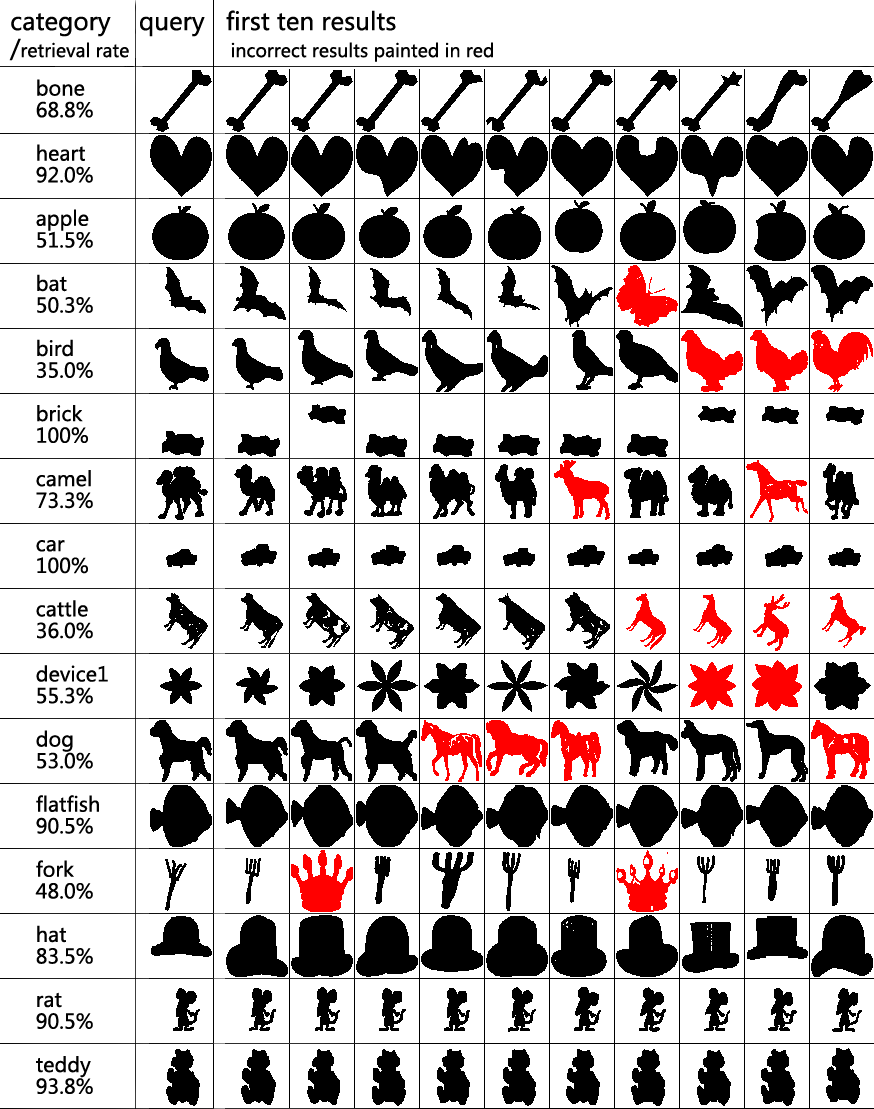
\includegraphics[width=1\linewidth]{images/fig10.png}
\end{center}
\caption{Shape retrieval on MPEG-7 shape data.} 
\label{fig:10}
\end{figure}

Some of the results are shown in \figurename~\ref{fig:10}.
We list the first ten results for each query and the incorrect ones are marked in red color.
The model made mistakes when the categories are similar, such as bird and chicken, or bat and butterfly.
The average performance over the whole data set is 63.9\%.
The model achieved 100\% retrieval rate in 8 categories.
Although this result is far from perfect compared with the best reported result \cite{bai2010},
the model is attractive for its connection with the mechanism of the visual cortex.
In the following subsection, we demonstrate that this model provides explanation
for the response pattern of V4 neurons.

\subsection{Simulating V4 Response}

Recent research shows that early orientation signals from the primary visual cortex
are synthesized into curved contour fragment representations in visual area V4 \cite{yau2012}.
Our model also synthesizes the output of simple units which extract orientation features from the input image.
We simulate the response of V4 neurons to curve segments that was used in biological experiments.
The set of curve segments is shown in \figurename~\ref{fig:11}(b).
They vary in curvature and angular orientation.

\begin{figure}[ht]
\begin{center}
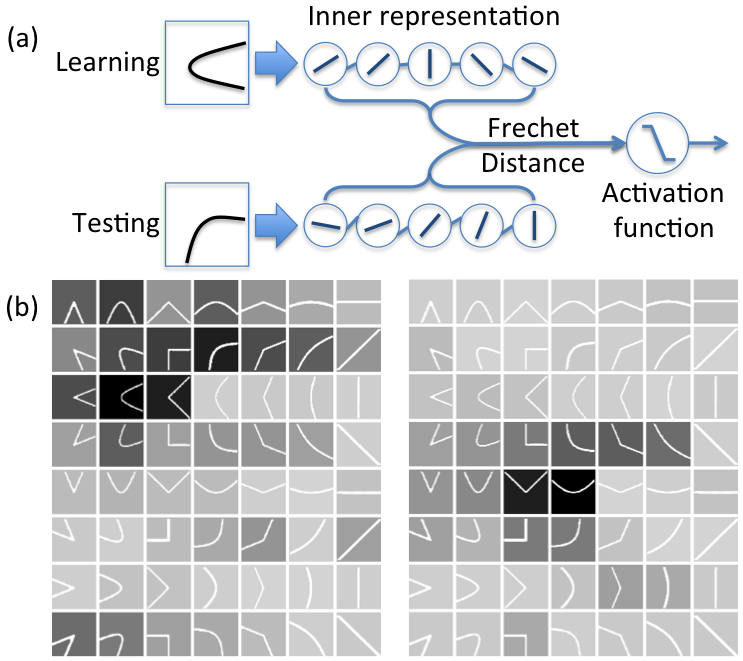
\includegraphics[width=0.98\linewidth]{images/fig11.png}
\end{center}
\caption{Simulating the response map of V4 neurons.
(a)~Matching curve segments with our model.
(b)~Simulated response map of V4 neurons.} 
\label{fig:11}
\end{figure}

To recognize a certain type of curve segment,
we store its representation with our model.
When presented with testing curve segments,
we calculate the Fr\'echet distance 
and use a step function to decide whether the simulated V4 neuron shall be activated.
\figurename~\ref{fig:11}(b) shows two simulated neurons
which respond to protruding curves towards the left and the bottom respectively.

\section{Conclusion}

In this paper, we present a novel model for contour representation and shape matching.
It is based on the orientation columns in the visual cortex.
Inspired by the way in which simple cells aggregate ganglion cells output,
we follow the hierarchical information processing mechanism of the cortex
and propose a new kind of contour representation by chaining activated simple computation units.
Using a modified version of discrete Fr\'echet distance,
we also provide a very efficient algorithm to compare the simple unit chain representations of contour lines
and thus make match between closed shapes.

We have further evaluated our model in shape retrieval experiment and V4 response simulation.
The model is highlighted for its connection with the shape selectivity found in the neurons of visual area V4. 
Future work would involve modeling of V4 neurons and representation of more complex shapes.

%\section{Acknowledgments}

\bibliographystyle{apacite}

\setlength{\bibleftmargin}{.125in}
\setlength{\bibindent}{-\bibleftmargin}

\bibliography{refs}


\end{document}
